\section{Verity Framework}

The Verity credibility graph models information as a network of sources and claims. We can define it as:

\[
G = (S, C, E)
\]

where \(S\) is the set of sources, \(C\) is the set of claims, and \(E\) is the set of assertions that connect sources to the claims they assert. This allows for a graph representation of how information is distributed across independent publishers. We use this graph as the foundation for credibility inference throughout the framework.

\subsection{Sources}

A source refers to an individual publisher that asserts one or more claims. Examples of sources may include websites, organizations, and databases. Every source is mapped to a unique node in the credibility graph.

\subsection{Claims}

A claim refers to a piece of information about an underlying entity. The same claim may be asserted by multiple different sources. Whereas other sources may assert conflicting claims about that same entity. Claims form nodes that connect different sources within the credibility graph.

\subsection{Assertions}

An assertion refers to the relationship between a source and a claim. Assertions are created every time a source asserts a claim which connects the corresponding source node to the claim node. These assertions form the overall graph structure and show how claims are distributed among many sources.

\subsection{Credibility Graph}

The credibility graph is made up of two types of nodes: sources and claims. Assertions connect these node types to form a bipartite graph. Sources connect only with claims and claims only connect with sources. Figure~\ref{fig:credibility-graph} illustrates a simplified example of the graph.

\begin{figure}[ht]
    \centering
    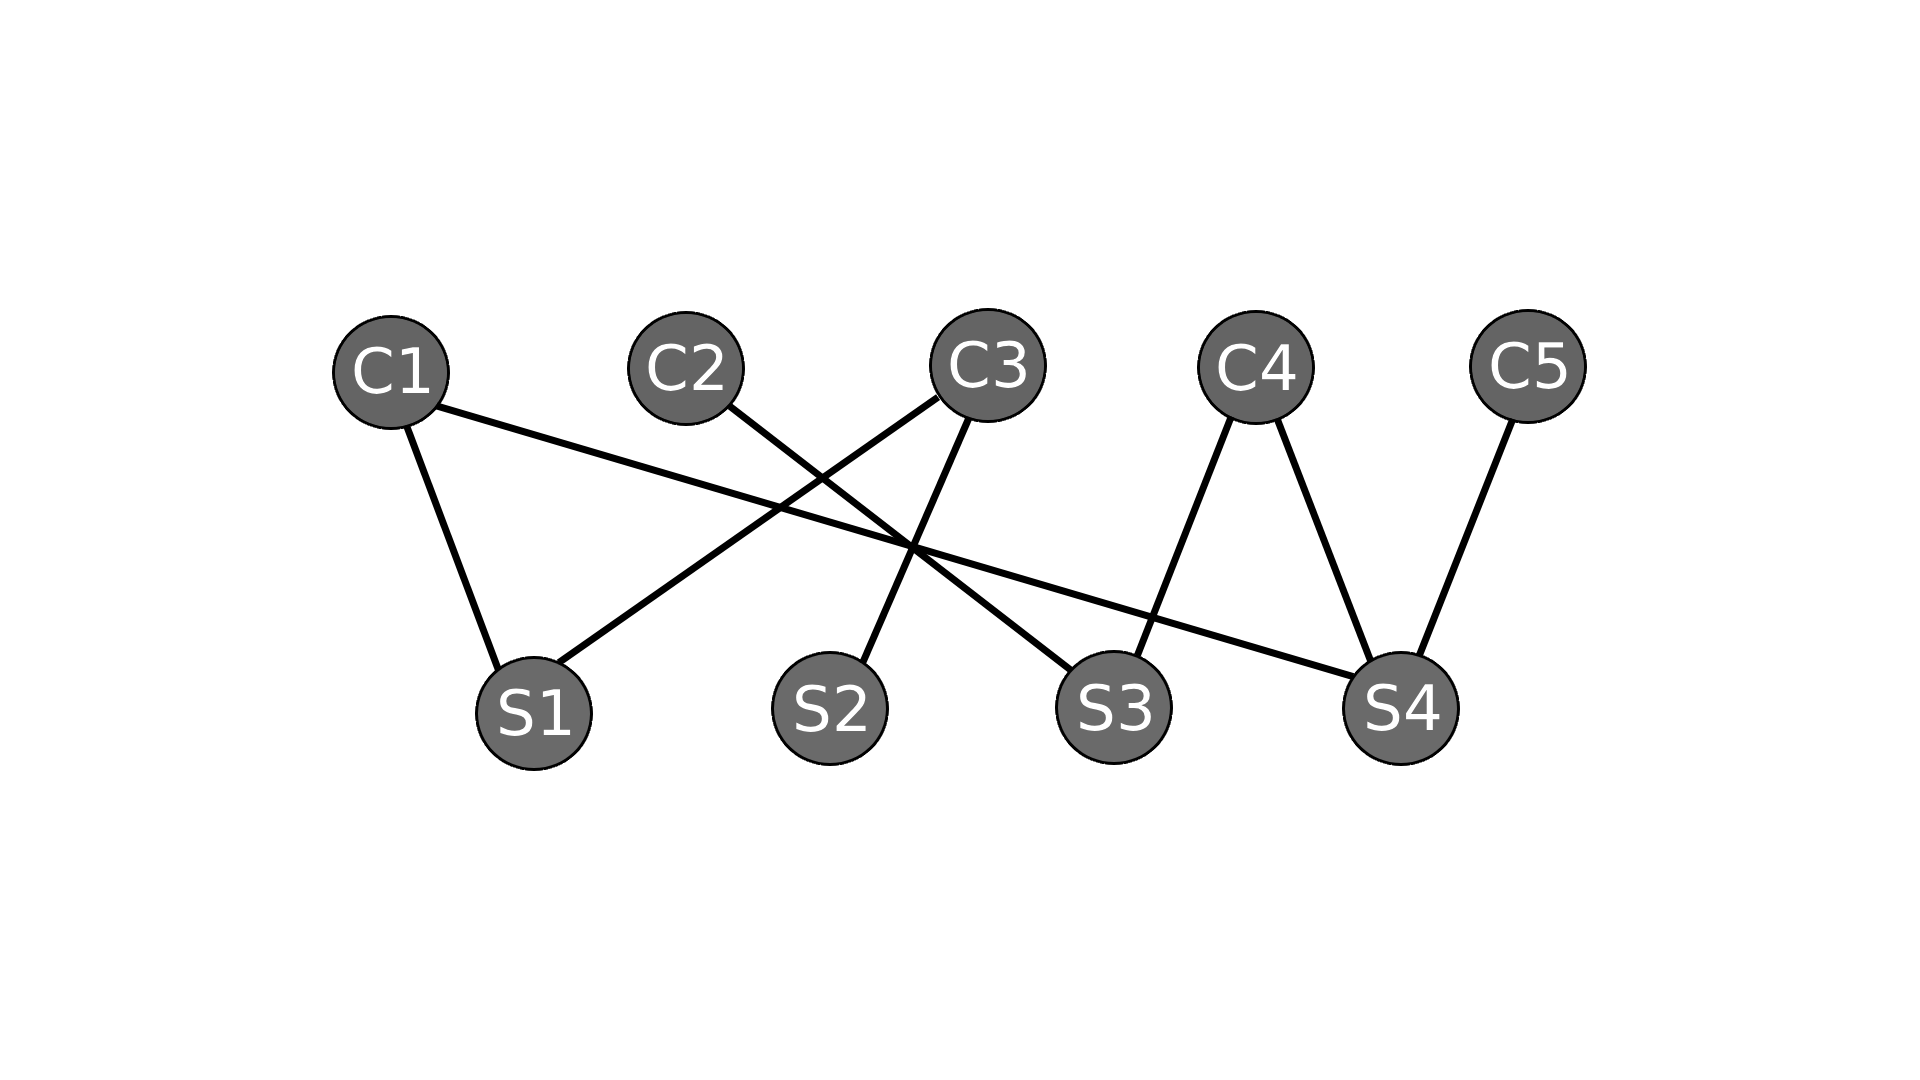
\includegraphics[width=0.8\textwidth]{figures/credibility_graph.png}
    \caption{Source nodes (red) are connected to the claim nodes (blue) they assert. Each edge represents one assertion.}
    \label{fig:credibility-graph}
\end{figure}
